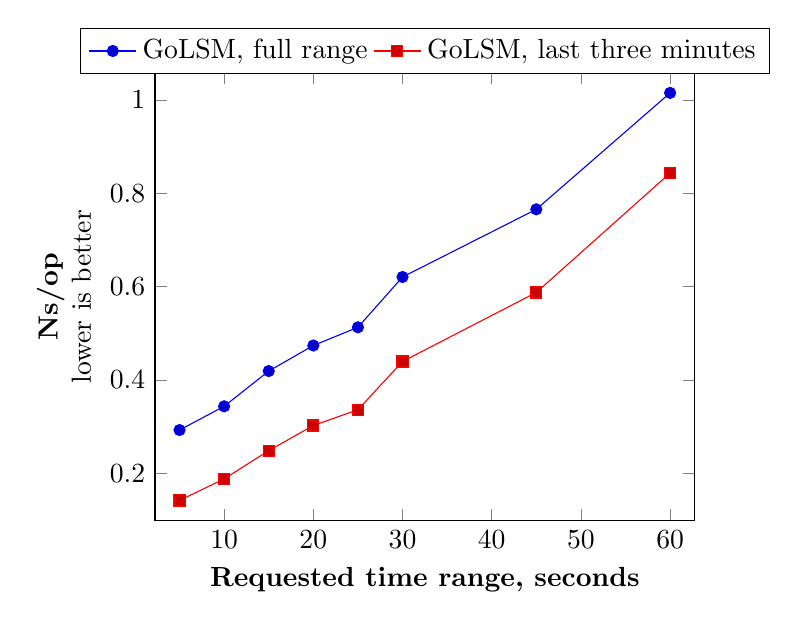
\begin{tikzpicture}
        % first provide your data as table, so later the data can
        % easily be accessed for various stuff
        \pgfplotstableread{
            x    y  z
5	29245	14164
10	34331	18772
15	41885	24835
20	47359	30221
25	51261	33592
30	62037	43931
45	76538	58727
60	101490	84315
        }{\data}
    \begin{axis}[
        x tick style={/pgf/number format/1000 sep=},
	    ylabel style={align=center},	
	    ylabel = \textbf{Ns/op}\\lower is better,
	    xlabel style={align=center},	
	    xlabel = \textbf{Requested time range, seconds},
	    enlargelimits=0.05,
	    legend style={
	        at={(0.5,1.1)}, anchor=north,legend columns=-1
	    },
    ]
        % then your `\addplot commands change to
        \addplot table [x=x,y=y] {\data};
        \addlegendentry{GoLSM, full range}
        \addplot table [x=x,y=z] {\data};
        \addlegendentry{GoLSM, last three minutes}
    \end{axis}
\end{tikzpicture}